\hypertarget{appendix-a8f634b076b5}{}
\section*{University - Graphics Vision and Photography - Visual Recall}
\chapter{Worlds, Images and Inference --- Fast Recall}\label{appendix-a8f634b076b5-worlds-images-and-inference-fast-recall}

\section{Fast route}\label{appendix-a8f634b076b5-fast-route}

Start with a world description and follow it through the physical and computational steps that form an image. Then ask what the measurements let us recover about the world. Each step changes representation and may discard information.

\pandocbounded{\includegraphics[keepaspectratio,alt={Diagram}]{/Users/swayamsingal/Library/Mobile Documents/iCloud~md~obsidian/Documents/Master/Book Production/AllMight Codex/QA/print-reference-dedup/assets/print/d057ccd2c6dd7ed7543b9acdc5019d6341d1b19bdf59cea25f3a640114dac8b5.pdf}}

\begin{enumerate}
\def\labelenumi{\arabic{enumi}.}
\tightlist
\item
  \textbf{Represent} points, curves, surfaces, and meshes with the data each operation needs.
\item
  \textbf{Place and move} geometry with coordinate frames, hierarchies, animation, and simulation.
\item
  \textbf{Measure} the scene through optics, exposure, sensors, and camera projection.
\item
  \textbf{Render} visible surfaces, material response, and light transport; rasterization and ray queries organize the work differently.
\item
  \textbf{Sample} the continuous image with filters and finite pixels, then encode color for a device.
\item
  \textbf{Infer} hidden motion, orientation, shape, or object pose from measurements, stating ambiguities and assumptions.
\end{enumerate}

For the core visual anchors, open \href{Continuous\%20Notes/University\%20-\%20Worlds,\%20Images\%20and\%20Inference\%20-\%20Graphics,\%20Vision\%20and\%20Photography\#Figure\%20U1\%20-\%20Linear\%20maps\%20separate\%20directions\%20stretches\%20and\%20output\%20placement}{Figure U1}; \href{Continuous\%20Notes/University\%20-\%20Worlds,\%20Images\%20and\%20Inference\%20-\%20Graphics,\%20Vision\%20and\%20Photography\#Figure\%20U2\%20-\%20A\%20half-edge\%20separates\%20face\%20traversal\%20from\%20edge\%20traversal}{Figure U2}; \href{Continuous\%20Notes/University\%20-\%20Worlds,\%20Images\%20and\%20Inference\%20-\%20Graphics,\%20Vision\%20and\%20Photography\#Figure\%20U3\%20-\%20Two\%20signals\%20can\%20share\%20the\%20same\%20samples}{Figure U3}; \href{Continuous\%20Notes/University\%20-\%20Worlds,\%20Images\%20and\%20Inference\%20-\%20Graphics,\%20Vision\%20and\%20Photography\#Figure\%20U4\%20-\%20Lighting\%20rank\%20determines\%20which\%20normal\%20components\%20can\%20be\%20measured}{Figure U4}; and \href{Continuous\%20Notes/University\%20-\%20Worlds,\%20Images\%20and\%20Inference\%20-\%20Graphics,\%20Vision\%20and\%20Photography\#Figure\%20U5\%20-\%20A\%20direct-light\%20renderer\%20makes\%20the\%20pipeline\%20executable}{Figure U5}.

\section{Thirty-five retrieval briefs}\label{appendix-a8f634b076b5-thirty-five-retrieval-briefs}

Each brief gives a mechanism to recall, the condition that matters, and a concrete question to use when reopening that section. The links target the matching chapter in the main note.

\begin{enumerate}
\def\labelenumi{\arabic{enumi}.}
\item
  \textbf{\href{Continuous\%20Notes/University\%20-\%20Worlds,\%20Images\%20and\%20Inference\%20-\%20Graphics,\%20Vision\%20and\%20Photography\#A\%20scene\%20description\%20becomes\%20an\%20image}{A scene description becomes an image}} --- Graphics maps a scene description to image measurements; vision works backward from measurements to constraints on the scene. Both depend on camera, geometry, light, and sampling assumptions. \textbf{Ask:} In a ray renderer and a rasterizer, which direction does the visibility query travel?
\item
  \textbf{\href{Continuous\%20Notes/University\%20-\%20Worlds,\%20Images\%20and\%20Inference\%20-\%20Graphics,\%20Vision\%20and\%20Photography\#Mathematical\%20language:\%20points,\%20vectors,\%20and\%20derivatives}{Mathematical language: points, vectors, and derivatives}} --- A point locates; a vector displaces. In a skew basis, geometric squared length is \(c^T Gc\), with \(G=B^TB\). A Jacobian predicts local change; the Hessian records curvature. \textbf{Ask:} Why does summing squared coordinates fail when basis vectors are not orthogonal?
\item
  \textbf{\href{Continuous\%20Notes/University\%20-\%20Worlds,\%20Images\%20and\%20Inference\%20-\%20Graphics,\%20Vision\%20and\%20Photography\#Coordinate\%20frames,\%20transformations,\%20and\%20pose}{Coordinate frames, transformations, and pose}} --- Homogeneous coordinates let one matrix translate points while leaving direction vectors unchanged. For column vectors, \(TS\) means scale first, then translate; order matters. Normals use inverse-transpose under nonuniform scale. \textbf{Ask:} What result does \(ST\) produce for a point when translation is accidentally scaled too?
\item
  \textbf{\href{Continuous\%20Notes/University\%20-\%20Worlds,\%20Images\%20and\%20Inference\%20-\%20Graphics,\%20Vision\%20and\%20Photography\#Curves\%20as\%20controllable\%20functions}{Curves as controllable functions}} --- A cubic has four degrees of freedom: endpoint positions and endpoint tangents fit Hermite data. Bézier controls expose tangents; de Casteljau evaluates and subdivides exactly. \(C^1\) matches parameter speed as well as direction; \(G^1\) only matches tangent direction. \textbf{Ask:} Why can a visually tangent join still have a speed jump?
\item
  \textbf{\href{Continuous\%20Notes/University\%20-\%20Worlds,\%20Images\%20and\%20Inference\%20-\%20Graphics,\%20Vision\%20and\%20Photography\#Surfaces,\%20patches,\%20topology,\%20and\%20parameterization}{Surfaces, patches, topology, and parameterization}} --- A chart maps a parameter domain onto a surface; its partial derivatives span the tangent plane. A chart can distort or become singular even if the surface itself is regular. \textbf{Ask:} What condition on the two tangent vectors makes a parameterization lose a local direction?
\item
  \textbf{\href{Continuous\%20Notes/University\%20-\%20Worlds,\%20Images\%20and\%20Inference\%20-\%20Graphics,\%20Vision\%20and\%20Photography\#Meshes,\%20connectivity,\%20and\%20geometry\%20processing}{Meshes, connectivity, and geometry processing}} --- A mesh stores geometry plus adjacency. Half-edges encode directed edge pairs and make face and vertex neighborhoods traversable. Edits must preserve required topology and orientation. See \href{Continuous\%20Notes/University\%20-\%20Worlds,\%20Images\%20and\%20Inference\%20-\%20Graphics,\%20Vision\%20and\%20Photography\#Figure\%20U2\%20-\%20A\%20half-edge\%20separates\%20face\%20traversal\%20from\%20edge\%20traversal}{Figure U2}. \textbf{Ask:} After an edge flip, which adjacent face can become inverted if the new diagonal is geometrically invalid?
\item
  \textbf{\href{Continuous\%20Notes/University\%20-\%20Worlds,\%20Images\%20and\%20Inference\%20-\%20Graphics,\%20Vision\%20and\%20Photography\#Lens\%20optics,\%20focus,\%20and\%20image\%20formation}{Lens optics, focus, and image formation}} --- A thin lens maps object distance to image distance; defocus spreads a point into a blur circle. Acceptable focus depends on the blur tolerance and output scale, not a universal depth-of-field boundary. The added derivation estimates a focus interval of about 2.34--4.19 m for its stated setup. \textbf{Ask:} Which chosen circle-of-confusion threshold changes that interval?
\item
  \textbf{\href{Continuous\%20Notes/University\%20-\%20Worlds,\%20Images\%20and\%20Inference\%20-\%20Graphics,\%20Vision\%20and\%20Photography\#Exposure,\%20sensors,\%20and\%20dynamic\%20range}{Exposure, sensors, and dynamic range}} --- Exposure controls collected photons through aperture, shutter time, and sensitivity; equivalent brightness does not imply equivalent motion blur, depth of field, noise, or highlight headroom. Sensor readout and saturation add limits. \textbf{Ask:} If shutter time is halved and aperture widened one stop, what changes besides image brightness?
\item
  \textbf{\href{Continuous\%20Notes/University\%20-\%20Worlds,\%20Images\%20and\%20Inference\%20-\%20Graphics,\%20Vision\%20and\%20Photography\#Cameras,\%20projection,\%20and\%20calibration}{Cameras, projection, and calibration}} --- Pinhole projection \(x=fX/Z\) couples image scale to depth. Vanishing points constrain parallel directions; calibration estimates internal parameters and pose from known geometry. Orthographic projection is useful when depth variation is negligible or should not affect measured scale. \textbf{Ask:} Why can three orthogonal vanishing directions still leave a mirror-related calibration solution?
\item
  \textbf{\href{Continuous\%20Notes/University\%20-\%20Worlds,\%20Images\%20and\%20Inference\%20-\%20Graphics,\%20Vision\%20and\%20Photography\#Sampling\%20continuous\%20signals\%20and\%20image\%20formation}{Sampling continuous signals and image formation}} --- Sampling records finite values of a continuous signal. Frequencies above half the sample rate can alias to a lower pattern; prefilter before reducing resolution. Pixel-area averaging is already a weak low-pass filter. See \href{Continuous\%20Notes/University\%20-\%20Worlds,\%20Images\%20and\%20Inference\%20-\%20Graphics,\%20Vision\%20and\%20Photography\#Figure\%20U3\%20-\%20Two\%20signals\%20can\%20share\%20the\%20same\%20samples}{Figure U3}. \textbf{Ask:} How can two different sinusoids produce identical samples on one grid?
\item
  \textbf{\href{Continuous\%20Notes/University\%20-\%20Worlds,\%20Images\%20and\%20Inference\%20-\%20Graphics,\%20Vision\%20and\%20Photography\#Image\%20sampling,\%20filtering,\%20and\%20efficient\%20reconstruction}{Image sampling, filtering, and efficient reconstruction}} --- Reconstruction filters trade alias suppression, blur, and ringing. A texture Jacobian maps a pixel footprint into texture space; mipmaps suit near-isotropic footprints, anisotropic filters suit elongated ones. Integral images turn any axis-aligned box sum into four table reads after one cumulative pass. \textbf{Ask:} Why does an integral image not make an arbitrary convolution constant-time?
\item
  \textbf{\href{Continuous\%20Notes/University\%20-\%20Worlds,\%20Images\%20and\%20Inference\%20-\%20Graphics,\%20Vision\%20and\%20Photography\#Color\%20perception,\%20encoding,\%20and\%20display}{Color perception, encoding, and display}} --- Cone responses compress a spectrum into three values, so distinct spectra can be metamers. Display codes are often nonlinear: decode to linear light before averaging or compositing, then encode for display. Gamut bounds which responses a device can reproduce. \textbf{Ask:} Why does encoded midpoint 0.5 represent roughly 0.22 linear intensity under gamma 2.2?
\item
  \textbf{\href{Continuous\%20Notes/University\%20-\%20Worlds,\%20Images\%20and\%20Inference\%20-\%20Graphics,\%20Vision\%20and\%20Photography\#Light\%20measurement\%20and\%20radiometry}{Light measurement and radiometry}} --- Flux, irradiance, intensity, and radiance use different measures. For an area-light element, conversion from area density to solid-angle density uses \(|n_y\cdot(-\omega)|/r^2\). Use the same measure as the integral. \textbf{Ask:} Why does sampling an area light require both the inverse-square factor and the light-normal cosine?
\item
  \textbf{\href{Continuous\%20Notes/University\%20-\%20Worlds,\%20Images\%20and\%20Inference\%20-\%20Graphics,\%20Vision\%20and\%20Photography\#Reflectance,\%20BRDFs,\%20and\%20shading}{Reflectance, BRDFs, and shading}} --- A BRDF describes how incoming direction becomes outgoing radiance. Lambertian reflectance is constant at \(\rho/\pi\); mirrors are delta-like and glossy materials form lobes. \textbf{Ask:} Why can a smooth directional sampler fail to hit an ideal mirror reflection?
\item
  \textbf{\href{Continuous\%20Notes/University\%20-\%20Worlds,\%20Images\%20and\%20Inference\%20-\%20Graphics,\%20Vision\%20and\%20Photography\#The\%20rendering\%20equation\%20and\%20light\%20transport}{The rendering equation and light transport}} --- Outgoing radiance is emitted light plus visible reflected incoming radiance integrated over a hemisphere. Since incoming radiance comes from other surfaces, transport is coupled. A renderer makes this executable with visibility, BRDF, light, and accumulation. See \href{Continuous\%20Notes/University\%20-\%20Worlds,\%20Images\%20and\%20Inference\%20-\%20Graphics,\%20Vision\%20and\%20Photography\#Figure\%20U5\%20-\%20A\%20direct-light\%20renderer\%20makes\%20the\%20pipeline\%20executable}{Figure U5}. \textbf{Ask:} Which term becomes zero when geometry blocks a sampled direction?
\item
  \textbf{\href{Continuous\%20Notes/University\%20-\%20Worlds,\%20Images\%20and\%20Inference\%20-\%20Graphics,\%20Vision\%20and\%20Photography\#Numerical\%20integration\%20and\%20Monte\%20Carlo\%20estimation}{Numerical integration and Monte Carlo estimation}} --- For samples \(X\sim p\), estimate \(\int f(x)dx\) with the mean of \(f(X)/p(X)\). Importance sampling reduces estimator variance only when the density covers every contributing region. \textbf{Ask:} Why does quadrupling independent samples usually halve standard error rather than quarter it?
\item
  \textbf{\href{Continuous\%20Notes/University\%20-\%20Worlds,\%20Images\%20and\%20Inference\%20-\%20Graphics,\%20Vision\%20and\%20Photography\#Rasterization,\%20coverage,\%20and\%20depth}{Rasterization, coverage, and depth}} --- Rasterization tests projected primitives at pixel sample locations, interpolates attributes, then depth-tests. Exact edge coverage is an area integral; multisampling estimates it with subpixel tests. Perspective-correct interpolation compensates for the projection divide. \textbf{Ask:} What artifact appears if a checkerboard floor is linearly interpolated in screen space?
\item
  \textbf{\href{Continuous\%20Notes/University\%20-\%20Worlds,\%20Images\%20and\%20Inference\%20-\%20Graphics,\%20Vision\%20and\%20Photography\#Textures\%20and\%20surface\%20detail}{Textures and surface detail}} --- Texture is a signal over surface coordinates. Charts introduce seams and distortion; filtering must follow how that domain projects into each pixel. \textbf{Ask:} Why can one square mip level overblur a floor receding toward the horizon?
\item
  \textbf{\href{Continuous\%20Notes/University\%20-\%20Worlds,\%20Images\%20and\%20Inference\%20-\%20Graphics,\%20Vision\%20and\%20Photography\#Visibility\%20queries\%20and\%20ray\%20intersections}{Visibility queries and ray intersections}} --- A ray query asks which geometry intersects a path from an origin; hit parameters, barycentric coordinates, and surface orientation answer different parts of the intersection contract. \textbf{Ask:} What additional bound distinguishes a ray from a finite line segment?
\item
  \textbf{\href{Continuous\%20Notes/University\%20-\%20Worlds,\%20Images\%20and\%20Inference\%20-\%20Graphics,\%20Vision\%20and\%20Photography\#Acceleration\%20structures\%20and\%20robust\%20queries}{Acceleration structures and robust queries}} --- A BVH groups geometry in nested bounds. Traversal skips a node only when its bound cannot intersect the query, so bounds must conservatively contain descendants. Robust predicates matter near tangencies and degenerate geometry. \textbf{Ask:} What correctness failure follows from rounding a bound inward?
\item
  \textbf{\href{Continuous\%20Notes/University\%20-\%20Worlds,\%20Images\%20and\%20Inference\%20-\%20Graphics,\%20Vision\%20and\%20Photography\#Scene\%20graphs\%20and\%20articulated\%20geometry}{Scene graphs and articulated geometry}} --- A node's world transform composes parent and local transforms; skinning blends posed bone candidates using per-vertex weights. Linear blends can collapse volume when averaging opposing rotations. \textbf{Ask:} Why does applying the inverse bind transform preserve a vertex when current pose equals rest pose?
\item
  \textbf{\href{Continuous\%20Notes/University\%20-\%20Worlds,\%20Images\%20and\%20Inference\%20-\%20Graphics,\%20Vision\%20and\%20Photography\#Animation\%20curves\%20and\%20motion\%20paths}{Animation curves and motion paths}} --- A moving camera needs position and orientation, plus a valid up direction. Smooth position does not guarantee smooth orientation; rotation interpolation and time parameterization are separate choices. \textbf{Ask:} What makes the camera frame singular when view and up vectors align?
\item
  \textbf{\href{Continuous\%20Notes/University\%20-\%20Worlds,\%20Images\%20and\%20Inference\%20-\%20Graphics,\%20Vision\%20and\%20Photography\#Dynamics,\%20forces,\%20and\%20numerical\%20integration}{Dynamics, forces, and numerical integration}} --- Dynamics evolves state from forces or interaction rules; an integrator approximates continuous time with steps. Large steps can inject energy or destabilize springs and cloth. \textbf{Ask:} Why can explicit Euler make a spring oscillation grow even when the physical model conserves energy?
\item
  \textbf{\href{Continuous\%20Notes/University\%20-\%20Worlds,\%20Images\%20and\%20Inference\%20-\%20Graphics,\%20Vision\%20and\%20Photography\#Optimization,\%20constraints,\%20and\%20inverse\%20kinematics}{Optimization, constraints, and inverse kinematics}} --- Define variables, objective, constraints, and derivatives before solving. IK linearizes forward kinematics with a Jacobian; feasibility and conditioning govern whether a target is reachable and stable. \textbf{Ask:} What changes when the end-effector Jacobian loses rank?
\item
  \textbf{\href{Continuous\%20Notes/University\%20-\%20Worlds,\%20Images\%20and\%20Inference\%20-\%20Graphics,\%20Vision\%20and\%20Photography\#PDEs,\%20fields,\%20and\%20discrete\%20solvers}{PDEs, fields, and discrete solvers}} --- A PDE, spatial discretization, and boundary conditions together define a numerical problem. Choosing a mesh or basis changes the system matrix; boundary data is part of the model. \textbf{Ask:} Why can two solvers using the same interior equation produce different solutions at the boundary?
\item
  \textbf{\href{Continuous\%20Notes/University\%20-\%20Worlds,\%20Images\%20and\%20Inference\%20-\%20Graphics,\%20Vision\%20and\%20Photography\#Optical\%20flow\%20and\%20motion\%20from\%20images}{Optical flow and motion from images}} --- Brightness constancy yields one equation, \(I_xu+I_yv+I_t=0\), for two flow components. A local aperture therefore leaves motion along an edge ambiguous. \textbf{Ask:} What does a single straight edge constrain well, and which motion component remains unobserved?
\item
  \textbf{\href{Continuous\%20Notes/University\%20-\%20Worlds,\%20Images\%20and\%20Inference\%20-\%20Graphics,\%20Vision\%20and\%20Photography\#Edges,\%20contours,\%20and\%20subpixel\%20localization}{Edges, contours, and subpixel localization}} --- Blur spreads an ideal edge; fitting a response profile can estimate its center between pixels. Hough voting accumulates weak local evidence into a global line or shape hypothesis. \textbf{Ask:} Why can an edge's subpixel estimate shift when the blur model is wrong?
\item
  \textbf{\href{Continuous\%20Notes/University\%20-\%20Worlds,\%20Images\%20and\%20Inference\%20-\%20Graphics,\%20Vision\%20and\%20Photography\#Recognition,\%20templates,\%20and\%20industrial\%20matching}{Recognition, templates, and industrial matching}} --- Template matching searches over pose and transformation with a score chosen for expected noise and deformation. Coarse-to-fine search reduces cost; thresholds set tolerance, not truth. \textbf{Ask:} Why should an edge alignment score treat normal displacement differently from tangent displacement?
\item
  \textbf{\href{Continuous\%20Notes/University\%20-\%20Worlds,\%20Images\%20and\%20Inference\%20-\%20Graphics,\%20Vision\%20and\%20Photography\#Pose\%20estimation,\%20transforms,\%20and\%20robust\%20fitting}{Pose estimation, transforms, and robust fitting}} --- Estimate rigid pose from correspondences, enforce a proper rotation, and use robust fitting when outliers contaminate matches. RANSAC trial count depends on inlier rate and sample size. \textbf{Ask:} Why does lowering the assumed inlier fraction sharply increase the number of RANSAC trials?
\item
  \textbf{\href{Continuous\%20Notes/University\%20-\%20Worlds,\%20Images\%20and\%20Inference\%20-\%20Graphics,\%20Vision\%20and\%20Photography\#Stereo,\%20relative\%20orientation,\%20and\%20reconstruction}{Stereo, relative orientation, and reconstruction}} --- Two views constrain rays and relative pose; triangulation recovers structure up to gauge freedoms such as global scale. Critical surfaces make the geometry ill-conditioned. \textbf{Ask:} Why can perfect image correspondences still leave metric scale unknown?
\item
  \textbf{\href{Continuous\%20Notes/University\%20-\%20Worlds,\%20Images\%20and\%20Inference\%20-\%20Graphics,\%20Vision\%20and\%20Photography\#Surface\%20orientation\%20from\%20illumination}{Surface orientation from illumination}} --- Photometric stereo uses several known light directions to solve for scaled normal from brightness measurements. The lighting matrix must span the components being estimated. See \href{Continuous\%20Notes/University\%20-\%20Worlds,\%20Images\%20and\%20Inference\%20-\%20Graphics,\%20Vision\%20and\%20Photography\#Figure\%20U4\%20-\%20Lighting\%20rank\%20determines\%20which\%20normal\%20components\%20can\%20be\%20measured}{Figure U4}. \textbf{Ask:} Which normal component becomes unobservable if every light direction lies in one plane?
\item
  \textbf{\href{Continuous\%20Notes/University\%20-\%20Worlds,\%20Images\%20and\%20Inference\%20-\%20Graphics,\%20Vision\%20and\%20Photography\#Shape\%20from\%20shading\%20and\%20reflectance}{Shape from shading and reflectance}} --- A single shading image gives a nonlinear relation among surface normal, reflectance, and illumination; integration into height requires boundary conditions and extra assumptions. \textbf{Ask:} Why does a locally valid normal field fail to guarantee one globally consistent surface?
\item
  \textbf{\href{Continuous\%20Notes/University\%20-\%20Worlds,\%20Images\%20and\%20Inference\%20-\%20Graphics,\%20Vision\%20and\%20Photography\#Surface\%20descriptions\%20and\%20Gaussian\%20images}{Surface descriptions and Gaussian images}} --- A Gaussian image maps surface area to normal directions. Its directional mass distribution summarizes orientation and curvature patterns but can be shared by geometrically different surfaces. \textbf{Ask:} Why does the zero-centroid condition hold for a closed surface, and what does it rule out?
\item
  \textbf{\href{Continuous\%20Notes/University\%20-\%20Worlds,\%20Images\%20and\%20Inference\%20-\%20Graphics,\%20Vision\%20and\%20Photography\#Photographic\%20composition,\%20history,\%20and\%20communication}{Photographic composition, history, and communication}} --- Viewpoint, crop, sequence, and caption shape how a photograph functions as evidence or argument. A recorded scene is selected and framed, not a neutral inventory. \textbf{Ask:} What does a wide frame reveal that a close crop hides in the same documentary image?
\item
  \textbf{\href{Continuous\%20Notes/University\%20-\%20Worlds,\%20Images\%20and\%20Inference\%20-\%20Graphics,\%20Vision\%20and\%20Photography\#Photographic\%20workflow\%20and\%20integrated\%20decisions}{Photographic workflow and integrated decisions}} --- Trace a capture from scene spectrum through optics, exposure, sampling, processing, and display. Each stage can discard information or add artifacts; choose settings around the intended output. \textbf{Ask:} Which stage caused a moiré pattern, and what evidence distinguishes it from JPEG blocking?
\end{enumerate}

\section{Evidence and scope}\label{appendix-a8f634b076b5-evidence-and-scope}

The source ledger covers \textbf{88 entries: 70 requested lectures and 18 added sources}. Its evidence includes \textbf{86 published English automatic-caption tracks, one locally generated Whisper transcript for a technical lecture, one sampled showcase video, and 70 lecture PDFs matched to their course years}. Captions, notes, and sampled visuals support different claims; the legend records which evidence supports each entry.

These briefs are deliberately compact retrieval notes for a 35-chapter continuous treatment. They are not a transcript, a substitute for the worked derivations, or a claim that the entire companion fits on one physical page.

\section{Four more figures to redraw from memory}\label{appendix-a8f634b076b5-four-more-figures-to-redraw-from-memory}

\begin{itemize}
\tightlist
\item
\item
\item
\item
\end{itemize}

\section{New mechanisms to retrieve}\label{appendix-a8f634b076b5-new-mechanisms-to-retrieve}

A vertex buffer is a byte array interpreted by a draw command. The stride says how many bytes separate successive vertices; the attribute offset says where one field begins inside a vertex. \href{Continuous\%20Notes/University\%20-\%20Worlds,\%20Images\%20and\%20Inference\%20-\%20Graphics,\%20Vision\%20and\%20Photography\#Rasterization,\%20coverage,\%20and\%20depth}{Rasterization and vertex layout} · \href{Continuous\%20Notes/University\%20-\%20Worlds,\%20Images\%20and\%20Inference\%20-\%20Graphics,\%20Vision\%20and\%20Photography\#Figure\%20U10\%20-\%20Vertex\%20fetch\%20uses\%20a\%20stride\%20and\%20byte\%20offset}{U10}. \textbf{Ask:} For 24-byte float32 vertices with RGB after XYZ, what are the position stride and color offset?

A mathematical projection of a finite point set is a map to a line. Small image size means many collisions. Scale, spacing, and additive structure determine whether many directions can compress the same set. This is separate from a camera's projection matrix. \href{Continuous\%20Notes/University\%20-\%20Worlds,\%20Images\%20and\%20Inference\%20-\%20Graphics,\%20Vision\%20and\%20Photography\#Finite-field\%20projections\%20turn\%20image\%20size\%20into\%20collision\%20counts}{Finite-field collisions} · \href{Continuous\%20Notes/University\%20-\%20Worlds,\%20Images\%20and\%20Inference\%20-\%20Graphics,\%20Vision\%20and\%20Photography\#Real\%20projections\%20add\%20scale,\%20spacing,\%20and\%20incidence\%20geometry}{Real projection scales} · \href{Continuous\%20Notes/University\%20-\%20Worlds,\%20Images\%20and\%20Inference\%20-\%20Graphics,\%20Vision\%20and\%20Photography\#Figure\%20U11\%20-\%20Finite-grid\%20projections\%20expose\%20collision\%20counts}{U11}. \textbf{Ask:} Is the obstruction arithmetic, spatial clustering, or an incidence pattern?

A classifier maps an image representation to scores; a loss compares those scores with the target. The gradient sends a local change backward through each operation by the chain rule. Convolution shares a local filter over the image; attention instead builds content-dependent weights between tokens. \href{Continuous\%20Notes/University\%20-\%20Worlds,\%20Images\%20and\%20Inference\%20-\%20Graphics,\%20Vision\%20and\%20Photography\#Learning\%20a\%20visual\%20classifier\%20from\%20examples}{Learning basics} · \href{Continuous\%20Notes/University\%20-\%20Worlds,\%20Images\%20and\%20Inference\%20-\%20Graphics,\%20Vision\%20and\%20Photography\#Convolutional\%20models\%20preserve\%20image\%20neighborhoods}{CNNs} · \href{Continuous\%20Notes/University\%20-\%20Worlds,\%20Images\%20and\%20Inference\%20-\%20Graphics,\%20Vision\%20and\%20Photography\#Sequence\%20models\%20and\%20attention}{Attention}. \textbf{Ask:} Which shape changes at each layer, and where does the chain rule multiply upstream and local derivatives?

Dense prediction assigns an output to every pixel; detection also predicts object locations and categories. Video adds temporal alignment, motion, and compute cost. \href{Continuous\%20Notes/University\%20-\%20Worlds,\%20Images\%20and\%20Inference\%20-\%20Graphics,\%20Vision\%20and\%20Photography\#Predict\%20pixels\%20and\%20localize\%20objects}{Dense prediction and detection} · \href{Continuous\%20Notes/University\%20-\%20Worlds,\%20Images\%20and\%20Inference\%20-\%20Graphics,\%20Vision\%20and\%20Photography\#Video\%20adds\%20motion\%20and\%20temporal\%20cost}{Video}. \textbf{Ask:} Does the evaluation measure pixel accuracy, object matching, or temporal consistency?

Self-supervision creates training targets from the data; generative objectives instead define how a model represents or samples possible outputs. Evaluation must match the claim: reconstruction quality, likelihood, sample quality, and downstream usefulness are different measurements. \href{Continuous\%20Notes/University\%20-\%20Worlds,\%20Images\%20and\%20Inference\%20-\%20Graphics,\%20Vision\%20and\%20Photography\#Self-supervision\%20and\%20evaluation}{Self-supervision} · \href{Continuous\%20Notes/University\%20-\%20Worlds,\%20Images\%20and\%20Inference\%20-\%20Graphics,\%20Vision\%20and\%20Photography\#Generative\%20models\%20learn\%20distributions\%20and\%20samplers}{Generative models}. \textbf{Ask:} What observable target trains the model, and what test would falsify the capability claim?

NeRF represents a scene with a learned field queried along rays; Gaussian splatting stores explicit 3D elements and composites their projected contributions. A planar Gaussian gives a direct local surface normal, while 3D Gaussian splats need geometric regularization to recover reliable surfaces. \href{Continuous\%20Notes/University\%20-\%20Worlds,\%20Images\%20and\%20Inference\%20-\%20Graphics,\%20Vision\%20and\%20Photography\#Learned\%20representations\%20of\%203D\%20shape\%20and\%20scenes}{Learned 3D representations} · \href{Continuous\%20Notes/University\%20-\%20Worlds,\%20Images\%20and\%20Inference\%20-\%20Graphics,\%20Vision\%20and\%20Photography\#From\%20scene\%20representations\%20to\%20research\%20methods}{research methods} · \href{Continuous\%20Notes/University\%20-\%20Worlds,\%20Images\%20and\%20Inference\%20-\%20Graphics,\%20Vision\%20and\%20Photography\#Figure\%20U12\%20-\%20Volume\%20compositing\%20accumulates\%20visible\%20contributions}{U12} · \href{Continuous\%20Notes/University\%20-\%20Worlds,\%20Images\%20and\%20Inference\%20-\%20Graphics,\%20Vision\%20and\%20Photography\#Figure\%20U13\%20-\%20A\%20local\%20Gaussian\%20covariance\%20projects\%20to\%20an\%20ellipse}{U13}. \textbf{Ask:} Which representation is queried per ray and which is explicitly rasterized?

An environment map supplies incoming illumination by direction. ReSTIR uses weighted reservoirs to reuse light candidates, but the final estimator still needs correct proposal support and normalization. LoD changes also change geometry, so reused paths need a surface correspondence and its area Jacobian. \href{Continuous\%20Notes/University\%20-\%20Worlds,\%20Images\%20and\%20Inference\%20-\%20Graphics,\%20Vision\%20and\%20Photography\#Light\%20measurement\%20and\%20radiometry}{Image-based lighting} · \href{Continuous\%20Notes/University\%20-\%20Worlds,\%20Images\%20and\%20Inference\%20-\%20Graphics,\%20Vision\%20and\%20Photography\#Numerical\%20integration\%20and\%20Monte\%20Carlo\%20estimation}{Monte Carlo reuse} · \href{Continuous\%20Notes/University\%20-\%20Worlds,\%20Images\%20and\%20Inference\%20-\%20Graphics,\%20Vision\%20and\%20Photography\#Figure\%20U14\%20-\%20A\%20reservoir\%20selects\%20a\%20candidate\%20by\%20its\%20weight}{U14}. \textbf{Ask:} What distribution was each candidate drawn from, and what normalization makes reuse valid?

Mitsuba 2 shows how a renderer can change execution mode and differentiate through image formation. It is a 2019 Enoki-based system; its API details are historical and should not be treated as Mitsuba 3 guidance. \href{Continuous\%20Notes/University\%20-\%20Worlds,\%20Images\%20and\%20Inference\%20-\%20Graphics,\%20Vision\%20and\%20Photography\#The\%20rendering\%20equation\%20and\%20light\%20transport}{Differentiable rendering}. \textbf{Ask:} Which quantities are differentiated and which sampling decisions are held fixed?

ARAP editing alternates local rigid rotations with a global sparse position solve. Field-aligned remeshing uses orientation and position fields to guide edge direction and placement. \href{Continuous\%20Notes/University\%20-\%20Worlds,\%20Images\%20and\%20Inference\%20-\%20Graphics,\%20Vision\%20and\%20Photography\#Meshes,\%20connectivity,\%20and\%20geometry\%20processing}{Mesh processing}. \textbf{Ask:} Which part is local per vertex and which system is solved globally?

IPC combines a contact barrier with continuous collision detection and a feasibility-preserving line search. A positive barrier alone is not a proof that a finite time step cannot cross a contact. \href{Continuous\%20Notes/University\%20-\%20Worlds,\%20Images\%20and\%20Inference\%20-\%20Graphics,\%20Vision\%20and\%20Photography\#Dynamics,\%20forces,\%20and\%20numerical\%20integration}{Contact dynamics} · \href{Continuous\%20Notes/University\%20-\%20Worlds,\%20Images\%20and\%20Inference\%20-\%20Graphics,\%20Vision\%20and\%20Photography\#Figure\%20U15\%20-\%20The\%20contact\%20barrier\%20grows\%20near\%20zero\%20separation}{U15}. \textbf{Ask:} What checks the entire path between the current and proposed configurations?

\pandocbounded{\includegraphics[keepaspectratio,alt={Diagram}]{/Users/swayamsingal/Library/Mobile Documents/iCloud~md~obsidian/Documents/Master/Book Production/AllMight Codex/QA/print-reference-dedup/assets/print/24f4ed21bdc904d70f3180acfb2f1d301f19ac7acf63b76456eab614914ded2c.pdf}}

Read the loop as a diagnostic map: representation, forward model, objective, and evaluation can each limit the result. It is not a single training algorithm; Monte Carlo rendering and supervised learning use different estimators and losses.

\pandocbounded{\includegraphics[keepaspectratio,alt={Diagram}]{/Users/swayamsingal/Library/Mobile Documents/iCloud~md~obsidian/Documents/Master/Book Production/AllMight Codex/QA/print-reference-dedup/assets/print/fc1cc5c8058813de182c4b8b70ce3dd3f99dd17e53892b61a59a7178a8cdebf8.pdf}}

This rendering/inference loop joins the original image-formation chapters to learned 3D methods. The reverse arrow indicates an inference problem; it does not imply a unique reconstruction.

\section{Rendering, materials, transport --- retrieve the reasons}\label{appendix-a8f634b076b5-rendering-materials-transport-retrieve-the-reasons}

\begin{figure}
\centering
\pandocbounded{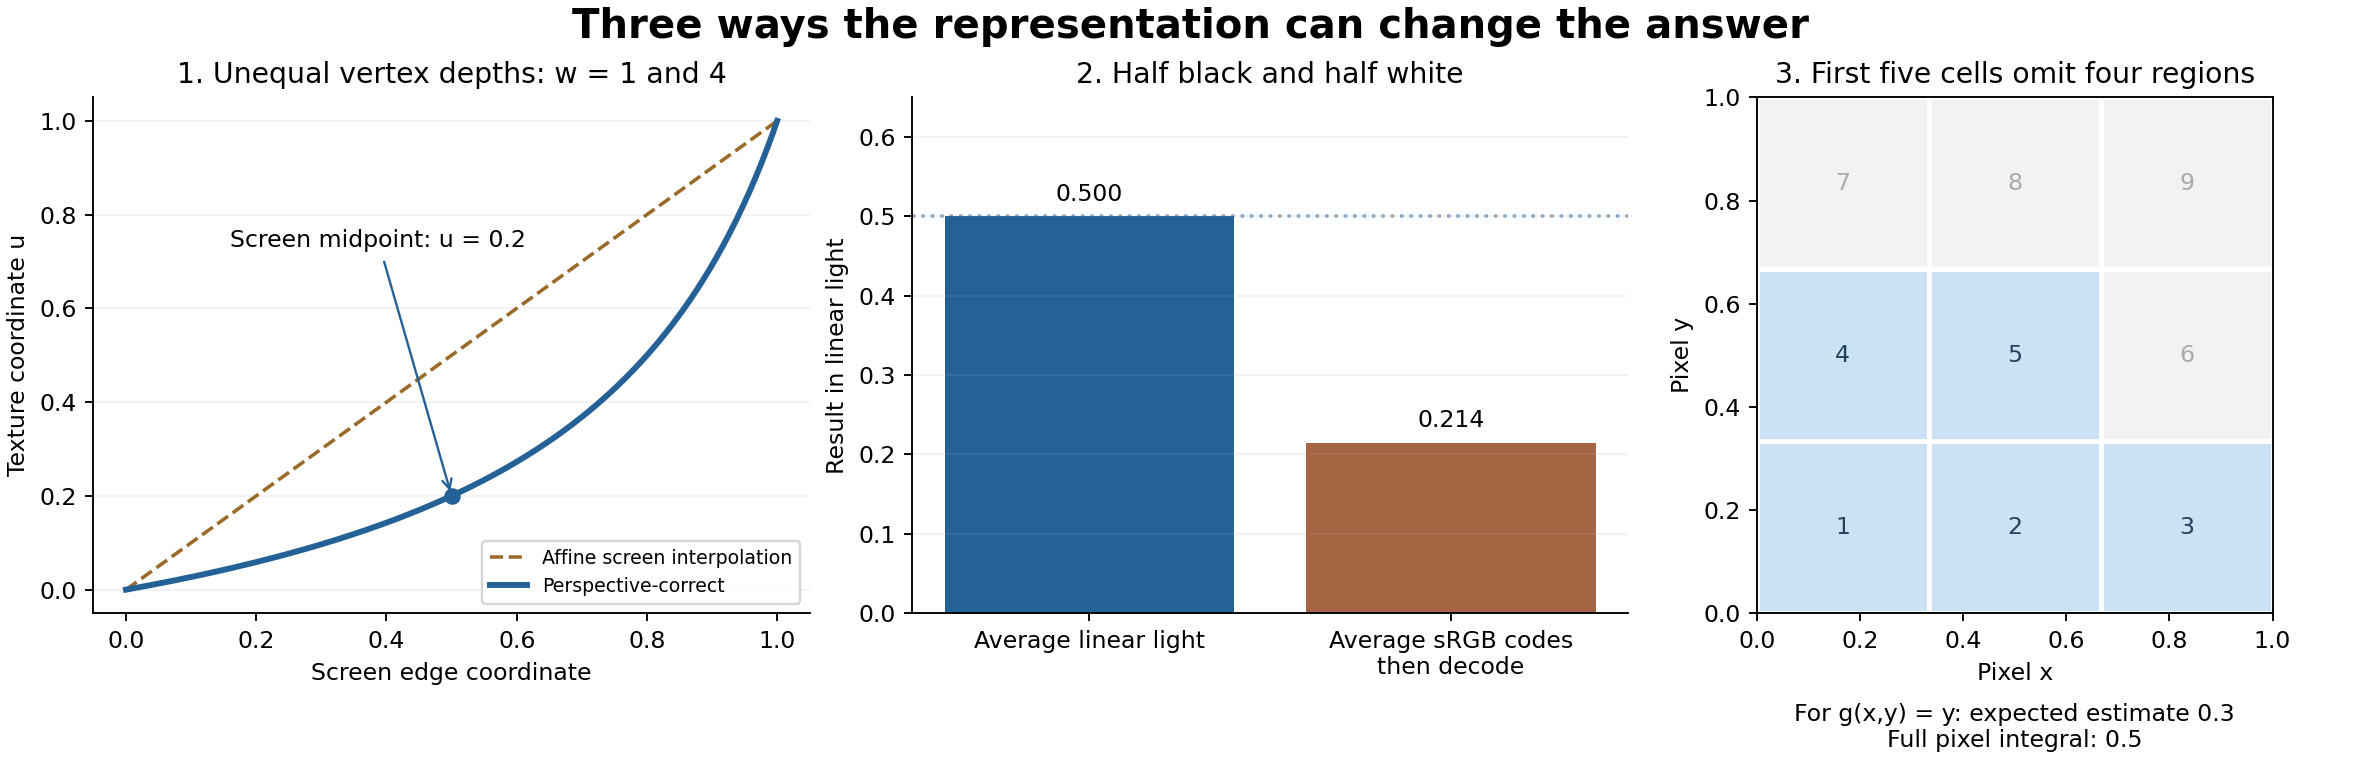
\includegraphics[keepaspectratio,alt={Visual Recall/Integrated Geometry and Engine/rendering-representation-witnesses.png}]{Visual Recall/Integrated Geometry and Engine/rendering-representation-witnesses.png}}
\caption{Visual Recall/Integrated Geometry and Engine/rendering-representation-witnesses.png}
\end{figure}

The left panel explains projective interpolation; the middle separates encoded storage from linear light; the right proves that a missing sampling region can create bias. These are numerical witnesses, not rendered screenshots from a working engine.

{\def\LTcaptype{none} % do not increment counter
\begin{longtable}[]{@{}
  >{\raggedright\arraybackslash}p{(\linewidth - 4\tabcolsep) * \real{0.3333}}
  >{\raggedright\arraybackslash}p{(\linewidth - 4\tabcolsep) * \real{0.3333}}
  >{\raggedright\arraybackslash}p{(\linewidth - 4\tabcolsep) * \real{0.3333}}@{}}
\toprule\noalign{}
\begin{minipage}[b]{\linewidth}\raggedright
Recall prompt
\end{minipage} & \begin{minipage}[b]{\linewidth}\raggedright
Short answer
\end{minipage} & \begin{minipage}[b]{\linewidth}\raggedright
Full teaching / figure explanation
\end{minipage} \\
\midrule\noalign{}
\endhead
\bottomrule\noalign{}
\endlastfoot
Why clip before dividing? & A primitive can cross the camera plane; division near zero creates unbounded coordinates. Clip the homogeneous primitive first. & {[}{[}Continuous Notes/University - Worlds, Images and Inference - Graphics, Vision and Photography\#Decide which samples a triangle owns \\
Which barycentrics recover a texture coordinate? & Screen weights need reciprocal-\(w\) correction. Already-divided depth instead interpolates affinely on screen. & {[}{[}Continuous Notes/University - Worlds, Images and Inference - Graphics, Vision and Photography\#Decide which samples a triangle owns \\
Why does reversed depth help? & Reciprocal distance pairs well with floating-point spacing near zero; every depth consumer must agree on ordering. & {[}{[}Continuous Notes/University - Worlds, Images and Inference - Graphics, Vision and Photography\#Give depth an explicit meaning \\
Why is encoded midpoint \(0.5\) too dark? & It decodes to about \(0.214\) linear light. Average linear values first. & {[}{[}Continuous Notes/University - Worlds, Images and Inference - Graphics, Vision and Photography\#Make every color number carry a meaning \\
What do \(D,F,G\) mean? & Facet distribution, interface reflection, and geometric visibility. The NDF normalizes with projected area. & {[}{[}Continuous Notes/University - Worlds, Images and Inference - Graphics, Vision and Photography\#Ask a surface where incoming energy can go \\
Why can a PDF exceed one? & It is density per unit measure. Its integral is one; its pointwise value need not be bounded by one. & {[}{[}Continuous Notes/University - Worlds, Images and Inference - Graphics, Vision and Photography\#Follow one path without losing its probability \\
What must area-light sampling include? & Light-choice probability, area density, and the area-to-solid-angle Jacobian. & {[}{[}Continuous Notes/University - Worlds, Images and Inference - Graphics, Vision and Photography\#Follow one path without losing its probability \\
What makes MIS complete? & Correctly weighted contributions from the participating sampling techniques, in the same measure, with delta events handled separately. & {[}{[}Continuous Notes/University - Worlds, Images and Inference - Graphics, Vision and Photography\#Follow one path without losing its probability \\
Does more sampling remove every error? & It reduces stochastic error under the estimator's assumptions. Missing-domain and transport-model bias can remain. & {[}{[}Continuous Notes/University - Worlds, Images and Inference - Graphics, Vision and Photography\#A missing region cannot be repaired by taking more samples there \\
\end{longtable}
}

Reconstruct without looking: show why the screen midpoint gives \(u=0.2\) for \(w=(1,4)\); derive the cosine hemisphere integral \(\pi\); convert a selected area-light density into solid angle; explain why roulette survivors divide by survival probability. Then point to where each assumption appears in the implementation.

\section{Explicit rendering, captured kernels and animated surfaces - retrieval briefs}\label{appendix-a8f634b076b5-explicit-rendering-captured-kernels-and-animated-surfaces---retrieval-briefs}

\begin{figure}
\centering
\pandocbounded{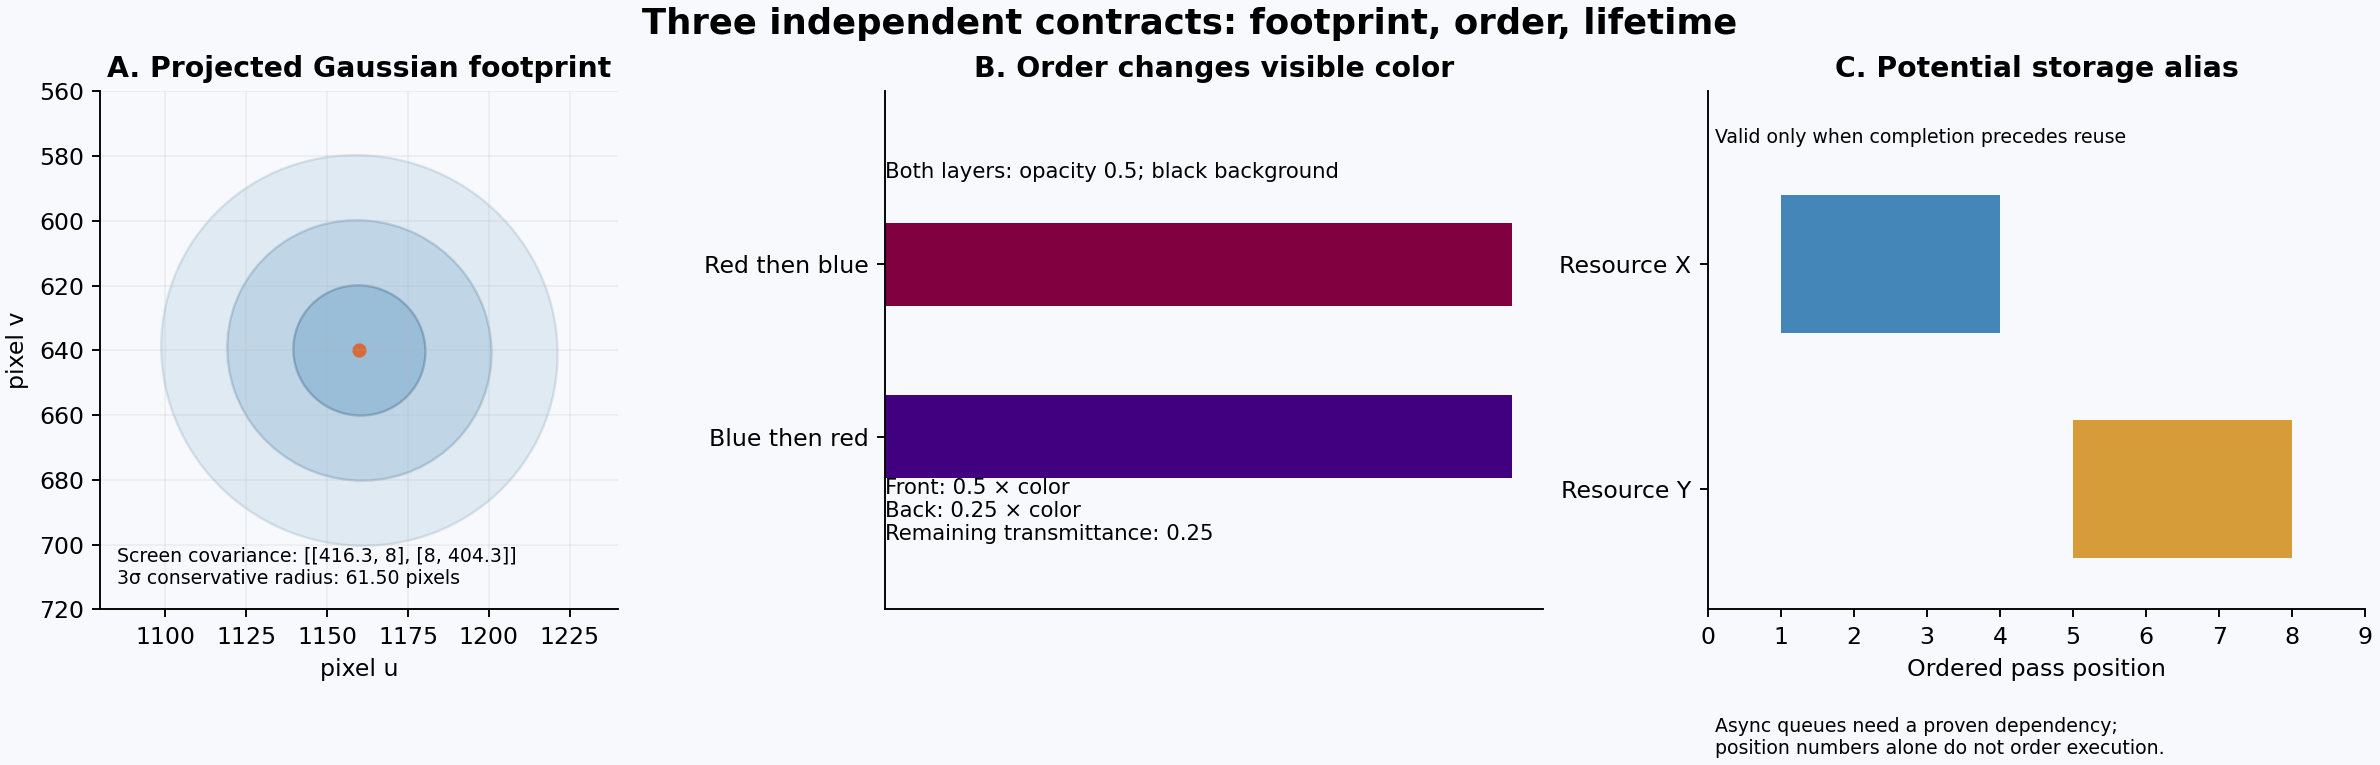
\includegraphics[keepaspectratio,alt={Visual Recall/Explicit Rendering/footprint-order-lifetime.png}]{Visual Recall/Explicit Rendering/footprint-order-lifetime.png}}
\caption{Visual Recall/Explicit Rendering/footprint-order-lifetime.png}
\end{figure}

\begin{itemize}
\item
  \textbf{\href{University\%20-\%20Worlds,\%20Images\%20and\%20Inference\%20-\%20Graphics,\%20Vision\%20and\%20Photography\#Local\%20projection\%20turns\%20an\%20ellipsoid\%20into\%20a\%20screen\%20ellipse}{Covariance to pixels}} --- A Jacobian is a local linear prediction. Transform covariance as \(J\Sigma J^T\), then invert the 2D covariance for the conic. Near-plane rejection and a finite footprint policy are prerequisites. Why is this only a local perspective approximation?
\item
  \textbf{\href{University\%20-\%20Worlds,\%20Images\%20and\%20Inference\%20-\%20Graphics,\%20Vision\%20and\%20Photography\#From\%20ellipses\%20to\%20bounded\%20tile\%20work}{Allocate tile work}} --- Count references, exclusive-scan counts, scatter to disjoint slices, sort by tile/depth, then composite. Counts \([4,2,5,1]\) give offsets \([0,4,6,11]\). Why must an unstable final tile sort not destroy depth order?
\item
  \textbf{\href{University\%20-\%20Worlds,\%20Images\%20and\%20Inference\%20-\%20Graphics,\%20Vision\%20and\%20Photography\#Figure\%20ER1\%20-\%20Footprint,\%20compositing\%20order\%20and\%20storage\%20lifetime}{Composite in order}} --- Contribution is \(T\alpha c\) and new transmittance is \(T(1-\alpha)\). Two half-opaque layers leave \(T=0.25\). A transmittance threshold is an approximation budget, not a universal reference constant.
\item
  \textbf{\href{University\%20-\%20Worlds,\%20Images\%20and\%20Inference\%20-\%20Graphics,\%20Vision\%20and\%20Photography\#Validation\%20should\%20isolate\%20representations\%20before\%20images}{Validate separate outputs}} --- Compare color in a declared space, depth with units, and IDs as discrete values. Average error, peak error and changed-pixel fraction answer different questions. CPU/GPU agreement does not establish antialiasing quality.
\item
  \textbf{\href{Computing\%20Foundations\%20-\%20From\%20Bits\%20to\%20C++\%20and\%20Systems\%20APIs\#Follow\%20a\%20frame\%20slot\%20and\%20a\%20presentation\%20image\%20separately}{Reuse the right object}} --- A slot fence proves slot work completed. It does not prove a presentation wait consumed its semaphore. Frame-slot and acquired-image indices are separate domains. What resolves an acquisition followed by recording failure?
\item
  \textbf{\href{Computing\%20Foundations\%20-\%20From\%20Bits\%20to\%20C++\%20and\%20Systems\%20APIs\#Retire\%20a\%20resource\%20after\%20every\%20user,\%20not\%20after\%20one\%20convenient\%20clock}{Retire across queues}} --- Every required queue counter must be reached. \((10,4,100)\) does not cover required \((9,5,3)\). Ownership preserves the payload; completion permits destruction.
\item
  \textbf{\href{Game\%20Engine\%20-\%20From\%20First\%20Frame\%20to\%20Living\%20Worlds\#2.\%20Compile\%20a\%20render\%20graph\%20before\%20executing\%20it}{Compile the graph}} --- Versions identify values, dependencies order producers/consumers, and lifetimes constrain storage aliasing. A list position does not prove that independent queues have stopped using memory.
\item
  \textbf{\href{Game\%20Engine\%20-\%20From\%20First\%20Frame\%20to\%20Living\%20Worlds\#Rendering\%20identity\%20becomes\%20world\%20identity\%20only\%20through\%20an\%20explicit\%20bridge}{Turn capture into editable world}} --- Persistent identity survives sorting; physical support supplies deformation. For affine motion, \(\mu'=F\mu+t\) and \(\Sigma'=F\Sigma F^T\). Appearance kernels alone supply neither mass nor colliders.
\item
  \textbf{\href{University\%20-\%20Worlds,\%20Images\%20and\%20Inference\%20-\%20Graphics,\%20Vision\%20and\%20Photography\#5.\%20Build\%20a\%20pose\%20first,\%20then\%20deform\%20the\%20surface}{Animate in a declared space}} --- Sample pose, resolve the hierarchy, morph before skinning, and build matching current/previous transforms. A global-joint palette already outputs world space. Why does adding the mesh world transform again break it?
\item
  \textbf{\href{Game\%20Engine\%20-\%20From\%20First\%20Frame\%20to\%20Living\%20Worlds\#An\%20image-change\%20certificate\%20must\%20name\%20the\%20edits\%20it\%20covers}{Image-change bounds need assumptions}} --- An opacity-only bound misses a red-to-blue edit at fixed opacity and a depth-order swap. State color range, evaluated per-pixel alpha changes, contributor order, color/background changes, and termination policy before calling an estimate a certificate.
\end{itemize}

\section{A moving pixel still needs a storage contract}\label{appendix-a8f634b076b5-a-moving-pixel-still-needs-a-storage-contract}

{\def\LTcaptype{none} % do not increment counter
\begin{longtable}[]{@{}
  >{\raggedright\arraybackslash}p{(\linewidth - 4\tabcolsep) * \real{0.3333}}
  >{\raggedright\arraybackslash}p{(\linewidth - 4\tabcolsep) * \real{0.3333}}
  >{\raggedright\arraybackslash}p{(\linewidth - 4\tabcolsep) * \real{0.3333}}@{}}
\toprule\noalign{}
\begin{minipage}[b]{\linewidth}\raggedright
Prompt
\end{minipage} & \begin{minipage}[b]{\linewidth}\raggedright
Short answer
\end{minipage} & \begin{minipage}[b]{\linewidth}\raggedright
Expand
\end{minipage} \\
\midrule\noalign{}
\endhead
\bottomrule\noalign{}
\endlastfoot
Flat index is valid; coordinates valid? & Not necessarily. At width 800, x=800,y=0 spills into the next row. Check each coordinate before indexing. & {[}{[}Continuous Notes/University - Worlds, Images and Inference - Graphics, Vision and Photography\#Animate a pixel by respecting the buffer's coordinates and lifetime \\
Cast a negative subpixel location? & Truncation can map -0.2 to 0; decide continuous clipping before conversion and reject nonfinite/out-of-range values. & {[}{[}Continuous Notes/University - Worlds, Images and Inference - Graphics, Vision and Photography\#Animate a pixel by respecting the buffer's coordinates and lifetime \\
Clear each frame or retain pixels? & Replacement frame versus intentional history. Clear once at the chosen frame boundary; define trail decay separately. & {[}{[}Continuous Notes/University - Worlds, Images and Inference - Graphics, Vision and Photography\#Animate a pixel by respecting the buffer's coordinates and lifetime \\
\end{longtable}
}

\section{Conservative culling: keep the region and the bound distinct}\label{appendix-a8f634b076b5-conservative-culling-keep-the-region-and-the-bound-distinct}

{\def\LTcaptype{none} % do not increment counter
\begin{longtable}[]{@{}
  >{\raggedright\arraybackslash}p{(\linewidth - 4\tabcolsep) * \real{0.3333}}
  >{\raggedright\arraybackslash}p{(\linewidth - 4\tabcolsep) * \real{0.3333}}
  >{\raggedright\arraybackslash}p{(\linewidth - 4\tabcolsep) * \real{0.3333}}@{}}
\toprule\noalign{}
\begin{minipage}[b]{\linewidth}\raggedright
Prompt
\end{minipage} & \begin{minipage}[b]{\linewidth}\raggedright
Short answer
\end{minipage} & \begin{minipage}[b]{\linewidth}\raggedright
Teaching / figure
\end{minipage} \\
\midrule\noalign{}
\endhead
\bottomrule\noalign{}
\endlastfoot
What does point-to-line distance measure? & Perpendicular distance to an infinite line; no endpoint, frustum or occlusion test. & {[}{[}Continuous Notes/University - Worlds, Images and Inference - Graphics, Vision and Photography\#A line corridor can be a cheap prefilter for shadow-caster work \\
When is rejecting a caster safe? & The corridor must enclose its possible contribution region; the object sphere must enclose transformed geometry. & {[}{[}Continuous Notes/University - Worlds, Images and Inference - Graphics, Vision and Photography\#A line corridor can be a cheap prefilter for shadow-caster work \\
Sphere radius 0.5, corridor radius 0.4? & Center distance above 0.9 rejects. A smaller distance only retains a candidate. & {[}{[}Visual Recall/Game Engine/corridor-and-shear.png \\
Largest matrix column bounds every stretch? & No under shear: a 1.414 guess misses a 1.618 stretch. Frobenius radius multiplier 2 is safe here. & {[}{[}Visual Recall/Game Engine/corridor-and-shear.svg \\
\end{longtable}
}

\textbf{Reconstruct:} prove the distance formula by parallelogram area; explain why an enclosing receiver corridor matters for directional shadows; show what breaks if scale or animation escapes the cached object bound.

\section{Mesh energy and value range}\label{appendix-a8f634b076b5-mesh-energy-and-value-range}

{\def\LTcaptype{none} % do not increment counter
\begin{longtable}[]{@{}
  >{\raggedright\arraybackslash}p{(\linewidth - 4\tabcolsep) * \real{0.3333}}
  >{\raggedright\arraybackslash}p{(\linewidth - 4\tabcolsep) * \real{0.3333}}
  >{\raggedright\arraybackslash}p{(\linewidth - 4\tabcolsep) * \real{0.3333}}@{}}
\toprule\noalign{}
\begin{minipage}[b]{\linewidth}\raggedright
Recall prompt
\end{minipage} & \begin{minipage}[b]{\linewidth}\raggedright
Short answer
\end{minipage} & \begin{minipage}[b]{\linewidth}\raggedright
Return to the teaching
\end{minipage} \\
\midrule\noalign{}
\endhead
\bottomrule\noalign{}
\endlastfoot
Can a negative cotangent edge weight coexist with nonnegative energy? & Yes. Valid element energies are squared gradients; individual signed edge terms are coupled by geometry. & {[}{[}Continuous Notes/University - Worlds, Images and Inference - Graphics, Vision and Photography\#Nonnegative energy and nonnegative weights are different promises \\
Does a stable heat step preserve nonnegative values? & Not necessarily: the worked step produces −0.015 while energy falls from 0.125 to 0.104525. & {[}{[}Continuous Notes/University - Worlds, Images and Inference - Graphics, Vision and Photography\#A stable heat step can still create a negative sample \\
What makes an explicit diffusion update a convex average? & Nonnegative edge weights, positive lumped masses, and a step small enough to keep every diagonal update coefficient nonnegative. & {[}{[}Continuous Notes/University - Worlds, Images and Inference - Graphics, Vision and Photography\#Complete single-triangle energy witness \\
\end{longtable}
}

\section{From measurements to state and pixels}\label{appendix-a8f634b076b5-from-measurements-to-state-and-pixels}

{\def\LTcaptype{none} % do not increment counter
\begin{longtable}[]{@{}
  >{\raggedright\arraybackslash}p{(\linewidth - 4\tabcolsep) * \real{0.3333}}
  >{\raggedright\arraybackslash}p{(\linewidth - 4\tabcolsep) * \real{0.3333}}
  >{\raggedright\arraybackslash}p{(\linewidth - 4\tabcolsep) * \real{0.3333}}@{}}
\toprule\noalign{}
\begin{minipage}[b]{\linewidth}\raggedright
Prompt
\end{minipage} & \begin{minipage}[b]{\linewidth}\raggedright
Short answer
\end{minipage} & \begin{minipage}[b]{\linewidth}\raggedright
Full commented reconstruction
\end{minipage} \\
\midrule\noalign{}
\endhead
\bottomrule\noalign{}
\endlastfoot
What makes the planar camera bearing model valid? & Known landmarks, planar motion and the explicitly identity body-to-camera extrinsic. & {[}{[}Continuous Notes/University - Worlds, Images and Inference - Graphics, Vision and Photography\#Make the visual correction small enough to inspect: an eight-state planar EKF \\
What is IMU preintegration compressing? & High-rate samples between keyframes into declared relative motion summaries; it is not a complete visual estimator. & {[}{[}Continuous Notes/University - Worlds, Images and Inference - Graphics, Vision and Photography\#From raw 3-D IMU samples to the pose constraint used by VIO \\
What connects extinction to a pixel? & Segment opacity and remaining transmittance weight emitted sample colors. & {[}{[}Continuous Notes/University - Worlds, Images and Inference - Graphics, Vision and Photography\#A NeRF pixel is an integral before it is a neural-network output \\
\end{longtable}
}

\section{Build a query structure without silently losing candidates}\label{appendix-a8f634b076b5-build-a-query-structure-without-silently-losing-candidates}

\pandocbounded{\includegraphics[keepaspectratio,alt={Diagram}]{/Users/swayamsingal/Library/Mobile Documents/iCloud~md~obsidian/Documents/Master/Book Production/AllMight Codex/QA/print-reference-dedup/assets/print/57cb8bfc0f9751c2a612ca0378027d15782a32c2fcf2702a7d702d1ed36bf794.pdf}}

Each arrow that transfers device-produced data needs the API's required dependency. Finishing a dispatch alone does not replace memory visibility.

{\def\LTcaptype{none} % do not increment counter
\begin{longtable}[]{@{}
  >{\raggedright\arraybackslash}p{(\linewidth - 4\tabcolsep) * \real{0.3333}}
  >{\raggedright\arraybackslash}p{(\linewidth - 4\tabcolsep) * \real{0.3333}}
  >{\raggedright\arraybackslash}p{(\linewidth - 4\tabcolsep) * \real{0.3333}}@{}}
\toprule\noalign{}
\begin{minipage}[b]{\linewidth}\raggedright
Recall prompt
\end{minipage} & \begin{minipage}[b]{\linewidth}\raggedright
Short answer
\end{minipage} & \begin{minipage}[b]{\linewidth}\raggedright
Full lesson
\end{minipage} \\
\midrule\noalign{}
\endhead
\bottomrule\noalign{}
\endlastfoot
Is an append ticket a stored record? & Only when it fits. Track attempted count, stored count and overflow; reject an incomplete candidate structure. & {[}{[}Continuous Notes/University - Worlds, Images and Inference - Graphics, Vision and Photography\#Build GPU bins and fixed hash tables only after capacity and ownership are explicit \\
How do bins avoid overlap? & Count entries, scan counts into disjoint starts, then scatter within each owned bin interval. Atomic arrival order can vary. & {[}{[}Continuous Notes/University - Worlds, Images and Inference - Graphics, Vision and Photography\#Worked 2D spatial-bin build \\
What does CAS publish in the small hash model? & It claims a key slot for one payload writer. Queries wait for the whole build and memory handoff. & {[}{[}Continuous Notes/University - Worlds, Images and Inference - Graphics, Vision and Photography\#Fixed-capacity open addressing with a bounded build pass \\
How does a full table terminate? & Probe at most its capacity; report failure and rebuild or reject. & {[}{[}Continuous Notes/University - Worlds, Images and Inference - Graphics, Vision and Photography\#Collision trace and full-table failure \\
\end{longtable}
}

\section{Buffering, budget and precision in five answers}\label{appendix-a8f634b076b5-buffering-budget-and-precision-in-five-answers}

{\def\LTcaptype{none} % do not increment counter
\begin{longtable}[]{@{}
  >{\raggedright\arraybackslash}p{(\linewidth - 4\tabcolsep) * \real{0.3333}}
  >{\raggedright\arraybackslash}p{(\linewidth - 4\tabcolsep) * \real{0.3333}}
  >{\raggedright\arraybackslash}p{(\linewidth - 4\tabcolsep) * \real{0.3333}}@{}}
\toprule\noalign{}
\begin{minipage}[b]{\linewidth}\raggedright
Prompt
\end{minipage} & \begin{minipage}[b]{\linewidth}\raggedright
Short answer
\end{minipage} & \begin{minipage}[b]{\linewidth}\raggedright
Return to the full derivation
\end{minipage} \\
\midrule\noalign{}
\endhead
\bottomrule\noalign{}
\endlastfoot
What retires a frame's storage? & Its final consumer's completed token; cycling a slot index proves nothing. & {[}{[}Continuous Notes/University - Worlds, Images and Inference - Graphics, Vision and Photography\#Double and triple buffering change ownership, not execution speed \\
Can async compute always overlap a draw? & Only if dependencies and resource contention permit. Two queues do not imply independent execution hardware. & {[}{[}Continuous Notes/University - Worlds, Images and Inference - Graphics, Vision and Photography\#Async compute starts with a dependency graph \\
Does persistent mapping permit overwrite? & No.~Mapping, cache visibility and consumer completion are different conditions. & {[}{[}Continuous Notes/University - Worlds, Images and Inference - Graphics, Vision and Photography\#Uploads need bandwidth, visibility and retirement \\
Which roofline ceiling matters? & The smaller of arithmetic peak and bandwidth × arithmetic intensity, with matching units and memory boundary. & {[}{[}Continuous Notes/University - Worlds, Images and Inference - Graphics, Vision and Photography\#Derive a roofline bound with matching units \\
Why can FP16 lose a unit increment at 2048? & Neighbor spacing is 2; 2049 rounds to 2048 under ties-to-even. Widening later cannot restore lost input. & {[}{[}Continuous Notes/University - Worlds, Images and Inference - Graphics, Vision and Photography\#Half precision is a range and accumulation decision \\
\end{longtable}
}

Reproduce the numerical examples in \href{Continuous\%20Notes/University\%20-\%20Worlds,\%20Images\%20and\%20Inference\%20-\%20Graphics,\%20Vision\%20and\%20Photography\#Check\%20the\%20scheduling\%20and\%20precision\%20examples\%20with\%20a\%20scalar\%20witness}{the six-check scalar witness}. The witness does not execute a GPU.
